% Options for packages loaded elsewhere
\PassOptionsToPackage{unicode}{hyperref}
\PassOptionsToPackage{hyphens}{url}
\PassOptionsToPackage{dvipsnames,svgnames,x11names}{xcolor}
%
\documentclass[
  letterpaper,
  DIV=11,
  numbers=noendperiod]{scrartcl}

\usepackage{amsmath,amssymb}
\usepackage{iftex}
\ifPDFTeX
  \usepackage[T1]{fontenc}
  \usepackage[utf8]{inputenc}
  \usepackage{textcomp} % provide euro and other symbols
\else % if luatex or xetex
  \usepackage{unicode-math}
  \defaultfontfeatures{Scale=MatchLowercase}
  \defaultfontfeatures[\rmfamily]{Ligatures=TeX,Scale=1}
\fi
\usepackage{lmodern}
\ifPDFTeX\else  
    % xetex/luatex font selection
\fi
% Use upquote if available, for straight quotes in verbatim environments
\IfFileExists{upquote.sty}{\usepackage{upquote}}{}
\IfFileExists{microtype.sty}{% use microtype if available
  \usepackage[]{microtype}
  \UseMicrotypeSet[protrusion]{basicmath} % disable protrusion for tt fonts
}{}
\makeatletter
\@ifundefined{KOMAClassName}{% if non-KOMA class
  \IfFileExists{parskip.sty}{%
    \usepackage{parskip}
  }{% else
    \setlength{\parindent}{0pt}
    \setlength{\parskip}{6pt plus 2pt minus 1pt}}
}{% if KOMA class
  \KOMAoptions{parskip=half}}
\makeatother
\usepackage{xcolor}
\setlength{\emergencystretch}{3em} % prevent overfull lines
\setcounter{secnumdepth}{-\maxdimen} % remove section numbering
% Make \paragraph and \subparagraph free-standing
\ifx\paragraph\undefined\else
  \let\oldparagraph\paragraph
  \renewcommand{\paragraph}[1]{\oldparagraph{#1}\mbox{}}
\fi
\ifx\subparagraph\undefined\else
  \let\oldsubparagraph\subparagraph
  \renewcommand{\subparagraph}[1]{\oldsubparagraph{#1}\mbox{}}
\fi


\providecommand{\tightlist}{%
  \setlength{\itemsep}{0pt}\setlength{\parskip}{0pt}}\usepackage{longtable,booktabs,array}
\usepackage{calc} % for calculating minipage widths
% Correct order of tables after \paragraph or \subparagraph
\usepackage{etoolbox}
\makeatletter
\patchcmd\longtable{\par}{\if@noskipsec\mbox{}\fi\par}{}{}
\makeatother
% Allow footnotes in longtable head/foot
\IfFileExists{footnotehyper.sty}{\usepackage{footnotehyper}}{\usepackage{footnote}}
\makesavenoteenv{longtable}
\usepackage{graphicx}
\makeatletter
\def\maxwidth{\ifdim\Gin@nat@width>\linewidth\linewidth\else\Gin@nat@width\fi}
\def\maxheight{\ifdim\Gin@nat@height>\textheight\textheight\else\Gin@nat@height\fi}
\makeatother
% Scale images if necessary, so that they will not overflow the page
% margins by default, and it is still possible to overwrite the defaults
% using explicit options in \includegraphics[width, height, ...]{}
\setkeys{Gin}{width=\maxwidth,height=\maxheight,keepaspectratio}
% Set default figure placement to htbp
\makeatletter
\def\fps@figure{htbp}
\makeatother

\KOMAoption{captions}{tableheading}
\makeatletter
\@ifpackageloaded{tcolorbox}{}{\usepackage[skins,breakable]{tcolorbox}}
\@ifpackageloaded{fontawesome5}{}{\usepackage{fontawesome5}}
\definecolor{quarto-callout-color}{HTML}{909090}
\definecolor{quarto-callout-note-color}{HTML}{0758E5}
\definecolor{quarto-callout-important-color}{HTML}{CC1914}
\definecolor{quarto-callout-warning-color}{HTML}{EB9113}
\definecolor{quarto-callout-tip-color}{HTML}{00A047}
\definecolor{quarto-callout-caution-color}{HTML}{FC5300}
\definecolor{quarto-callout-color-frame}{HTML}{acacac}
\definecolor{quarto-callout-note-color-frame}{HTML}{4582ec}
\definecolor{quarto-callout-important-color-frame}{HTML}{d9534f}
\definecolor{quarto-callout-warning-color-frame}{HTML}{f0ad4e}
\definecolor{quarto-callout-tip-color-frame}{HTML}{02b875}
\definecolor{quarto-callout-caution-color-frame}{HTML}{fd7e14}
\makeatother
\makeatletter
\makeatother
\makeatletter
\makeatother
\makeatletter
\@ifpackageloaded{caption}{}{\usepackage{caption}}
\AtBeginDocument{%
\ifdefined\contentsname
  \renewcommand*\contentsname{Table of contents}
\else
  \newcommand\contentsname{Table of contents}
\fi
\ifdefined\listfigurename
  \renewcommand*\listfigurename{List of Figures}
\else
  \newcommand\listfigurename{List of Figures}
\fi
\ifdefined\listtablename
  \renewcommand*\listtablename{List of Tables}
\else
  \newcommand\listtablename{List of Tables}
\fi
\ifdefined\figurename
  \renewcommand*\figurename{Figure}
\else
  \newcommand\figurename{Figure}
\fi
\ifdefined\tablename
  \renewcommand*\tablename{Table}
\else
  \newcommand\tablename{Table}
\fi
}
\@ifpackageloaded{float}{}{\usepackage{float}}
\floatstyle{ruled}
\@ifundefined{c@chapter}{\newfloat{codelisting}{h}{lop}}{\newfloat{codelisting}{h}{lop}[chapter]}
\floatname{codelisting}{Listing}
\newcommand*\listoflistings{\listof{codelisting}{List of Listings}}
\makeatother
\makeatletter
\@ifpackageloaded{caption}{}{\usepackage{caption}}
\@ifpackageloaded{subcaption}{}{\usepackage{subcaption}}
\makeatother
\makeatletter
\@ifpackageloaded{tcolorbox}{}{\usepackage[skins,breakable]{tcolorbox}}
\makeatother
\makeatletter
\@ifundefined{shadecolor}{\definecolor{shadecolor}{rgb}{.97, .97, .97}}
\makeatother
\makeatletter
\makeatother
\makeatletter
\makeatother
\ifLuaTeX
  \usepackage{selnolig}  % disable illegal ligatures
\fi
\IfFileExists{bookmark.sty}{\usepackage{bookmark}}{\usepackage{hyperref}}
\IfFileExists{xurl.sty}{\usepackage{xurl}}{} % add URL line breaks if available
\urlstyle{same} % disable monospaced font for URLs
\hypersetup{
  pdftitle={Completely Randomised Design},
  colorlinks=true,
  linkcolor={blue},
  filecolor={Maroon},
  citecolor={Blue},
  urlcolor={Blue},
  pdfcreator={LaTeX via pandoc}}

\title{Completely Randomised Design}
\author{}
\date{}

\begin{document}
\maketitle
\ifdefined\Shaded\renewenvironment{Shaded}{\begin{tcolorbox}[interior hidden, sharp corners, boxrule=0pt, frame hidden, borderline west={3pt}{0pt}{shadecolor}, enhanced, breakable]}{\end{tcolorbox}}\fi

\renewcommand*\contentsname{Table of contents}
{
\hypersetup{linkcolor=}
\setcounter{tocdepth}{3}
\tableofcontents
}
In the \textbf{1920s}, statistician {Ronald A. Fisher} made significant
contributions to the development of the \textbf{Completely Randomized
Design (CRD)}, which was first used in the early 20th century. Fisher
developed this design to enhance agricultural studies, particularly to
identify subtle yet significant variations in crop yields under various
fertilizer treatments. His novel approach was to \textbf{prevent bias}
and enable reliable \textbf{statistical analysis} through analysis of
variance \textbf{(ANOVA)} by randomly assigning treatments to
experimental units (like land plots). In order to prevent bias and
enable reliable statistical analysis using analysis of variance (ANOVA),
he invented the practice of randomly allocating treatments to
experimental units.

In this design,\textbf{experimental units} are randomly assigned to
\textbf{treatments} without any systematic bias, ensuring that every
unit has an equal probability of receiving any given treatment. This
random assignment helps counter potential biases and addresses the
inherent variability among experimental units, making comparisons
between treatments impartial. In order to account for \textbf{natural
variation} in soil and environment, the first famous instances involved
agricultural field trials in which adjacent plots were randomly assigned
to different crop kinds or fertilizer treatments. \textbf{Agricultural
field trials} were the first well-known instances, in which adjacent
plots were randomly assigned to different crop varieties or fertilizer
treatments to account for inherent soil and environmental variance.

Although \textbf{CRD} is generally not advised for heterogeneous
settings, it is especially appropriate when the experimental material is
\textbf{homogeneous}, as in laboratory or greenhouse investigations. Due
to its ease of use and efficiency, CRD has established itself as a key
instrument in experimental statistics and is still essential in domains
including industrial engineering, quality control analysis, medicine,
and agriculture.

\begin{tcolorbox}[enhanced jigsaw, titlerule=0mm, title=\textcolor{quarto-callout-tip-color}{\faLightbulb}\hspace{0.5em}{This design is used to examine the effects of a single primary element
without considering additional bothersome aspects.}, bottomrule=.15mm, colback=white, opacityback=0, rightrule=.15mm, colframe=quarto-callout-tip-color-frame, toprule=.15mm, toptitle=1mm, leftrule=.75mm, left=2mm, arc=.35mm, breakable, coltitle=black, bottomtitle=1mm, colbacktitle=quarto-callout-tip-color!10!white, opacitybacktitle=0.6]

\end{tcolorbox}

\begin{figure}

{\centering 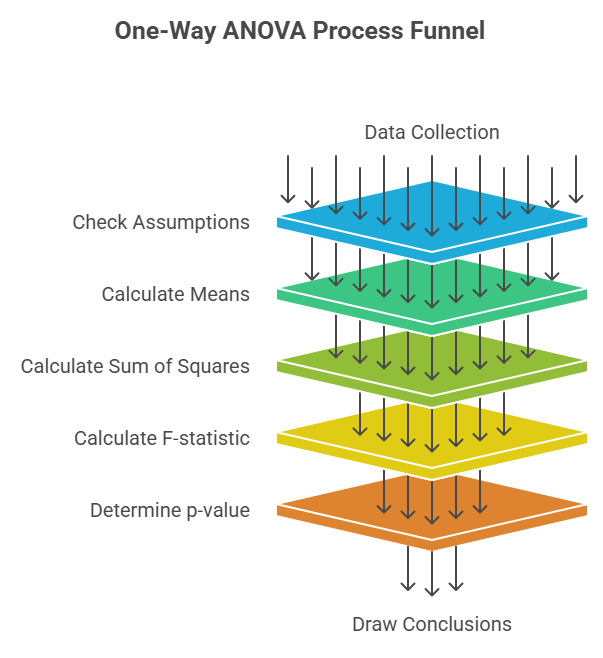
\includegraphics[width=5.32292in,height=\textheight]{onewayANOVA.png}

}

\end{figure}

\hypertarget{key-characteristics}{%
\section{Key Characteristics}\label{key-characteristics}}

Here are the main features of the design - hover or click each point to
see more information.

{🎲 Random allocation}

{🌿 Homogeneous conditions}

{🔄 Flexibility}

{📊 Simple analysis}

\hypertarget{sec-results}{%
\section{When to Use CRD? Explore Each Situation}\label{sec-results}}

\textbf{Below given are the appropriate situations to be used for CRD,
please click on each icon to see more information}

🧪 Laboratory Experiments

Best used under controlled conditions for reproducible results.

🌱 Greenhouse Experiments

Ideal for experiments where environmental uniformity is crucial.

🐄 Animal Feeding Trials

Works well when animals are homogeneous in age, breed, or weight.

🪴 Pot Experiments

Suitable for experiments with uniform soil and environmental factors.

\hypertarget{advantages-disadvantages-of-crd}{%
\section{Advantages \& Disadvantages of
CRD}\label{advantages-disadvantages-of-crd}}

\begin{tcolorbox}[enhanced jigsaw, titlerule=0mm, title={Advantages}, bottomrule=.15mm, colback=white, opacityback=0, rightrule=.15mm, colframe=quarto-callout-tip-color-frame, toprule=.15mm, toptitle=1mm, leftrule=.75mm, left=2mm, arc=.35mm, breakable, coltitle=black, bottomtitle=1mm, colbacktitle=quarto-callout-tip-color!10!white, opacitybacktitle=0.6]

• Simple to design and analyze\\
• Flexible in number of treatments and replications\\
• Maximum degrees of freedom for error term\\
• Missing data doesn't complicate analysis significantly\\
• Easy to understand and implement\\

\end{tcolorbox}

\begin{tcolorbox}[enhanced jigsaw, titlerule=0mm, title={Disadvantages}, bottomrule=.15mm, colback=white, opacityback=0, rightrule=.15mm, colframe=quarto-callout-warning-color-frame, toprule=.15mm, toptitle=1mm, leftrule=.75mm, left=2mm, arc=.35mm, breakable, coltitle=black, bottomtitle=1mm, colbacktitle=quarto-callout-warning-color!10!white, opacitybacktitle=0.6]

• Requires homogeneous experimental conditions\\
• Less precise than blocking designs when heterogeneity exists\\
• Can lead to larger experimental error if conditions are not uniform\\

\end{tcolorbox}

\hypertarget{layout-example}{%
\section{Layout Example}\label{layout-example}}

Suppose we're testing 4 fertilizer treatments (A, B, C, D) with 5
replications each (20 experimental units total) the \textbf{CRD Layout}
will be as given below.

\begin{figure}

{\centering \includegraphics{ssleg.webp}

}

\end{figure}

\hypertarget{crd-linear-model}{%
\section{CRD Linear Model}\label{crd-linear-model}}

The mathematical form of the \textbf{Completely Randomised Design (CRD)}
is very important because it gives a precise, structured way to describe
and analyze the experiment statistically. This helps us understand that
what we observe is not just random - it's a combination of systematic
treatment differences and random variation.

The \textbf{CRD linear model} allows us to partition the total variation
in the data into:

\begin{itemize}
\item
  Variation due to treatments
\item
  Variation due to random error
\end{itemize}

\textbf{The model assumes}: Errors are independent, normally
distributed, and have equal variance. These assumptions make it possible
to apply valid statistical tests, confidence intervals, and predictive
models.

\begin{tcolorbox}[enhanced jigsaw, titlerule=0mm, title={\textbf{CRD Linear Model}}, bottomrule=.15mm, colback=white, opacityback=0, rightrule=.15mm, colframe=quarto-callout-tip-color-frame, toprule=.15mm, toptitle=1mm, leftrule=.75mm, left=2mm, arc=.35mm, breakable, coltitle=black, bottomtitle=1mm, colbacktitle=quarto-callout-tip-color!10!white, opacitybacktitle=0.6]

Yij = μ + τi + εij

\end{tcolorbox}

Yij = observation for the jth unit receiving the ith treatment

μ = overall mean

τi = effect of the ith treatment

εij = random error (assumed \textasciitilde{} N(0, σ²))

i = 1, 2, \ldots, t (number of treatments)

j = 1, 2, \ldots, r (number of replications)

\begin{tcolorbox}[enhanced jigsaw, titlerule=0mm, title=\textcolor{quarto-callout-tip-color}{\faLightbulb}\hspace{0.5em}{Without the mathematical model, we couldn't formally test or compare
treatments reliably.}, bottomrule=.15mm, colback=white, opacityback=0, rightrule=.15mm, colframe=quarto-callout-tip-color-frame, toprule=.15mm, toptitle=1mm, leftrule=.75mm, left=2mm, arc=.35mm, breakable, coltitle=black, bottomtitle=1mm, colbacktitle=quarto-callout-tip-color!10!white, opacitybacktitle=0.6]

\end{tcolorbox}

\hypertarget{anova-table-for-completely-randomized-design-crd}{%
\section{ANOVA Table for Completely Randomized Design
(CRD)}\label{anova-table-for-completely-randomized-design-crd}}

\begin{longtable}[]{@{}
  >{\centering\arraybackslash}p{(\columnwidth - 8\tabcolsep) * \real{0.2241}}
  >{\centering\arraybackslash}p{(\columnwidth - 8\tabcolsep) * \real{0.2500}}
  >{\centering\arraybackslash}p{(\columnwidth - 8\tabcolsep) * \real{0.2155}}
  >{\centering\arraybackslash}p{(\columnwidth - 8\tabcolsep) * \real{0.1897}}
  >{\centering\arraybackslash}p{(\columnwidth - 8\tabcolsep) * \real{0.1207}}@{}}
\toprule\noalign{}
\begin{minipage}[b]{\linewidth}\centering
\textbf{Source of Variation}
\end{minipage} & \begin{minipage}[b]{\linewidth}\centering
\textbf{Degrees of Freedom (df)}
\end{minipage} & \begin{minipage}[b]{\linewidth}\centering
\textbf{Sum of Squares (SS)}
\end{minipage} & \begin{minipage}[b]{\linewidth}\centering
\textbf{Mean Square (MS)}
\end{minipage} & \begin{minipage}[b]{\linewidth}\centering
\textbf{F Ratio}
\end{minipage} \\
\midrule\noalign{}
\endhead
\bottomrule\noalign{}
\endlastfoot
Treatments & ( t - 1 ) & SST & MST & ( \dfrac{MST}{MSE} ) \\
Error (Residual) & ( N - t ) & SSE & MSE & \\
Total & ( N - 1 ) & TSS & & \\
\end{longtable}

\hypertarget{example}{%
\section{Example}\label{example}}

Let's explore some practical situations in agricultural research where
the Completely Randomised Design, also known as the CRD, is applied.

\hypertarget{sec-example}{%
\subsection{Study Context}\label{sec-example}}

\begin{enumerate}
\def\labelenumi{\arabic{enumi}.}
\tightlist
\item
  Ten mango cultivars, each representing a different treatment, are
  being evaluated by a horticultural scientist. Alphonso, Kesar,
  Dasheri, Himsagar, Chausa, Badami, Safeda, Bombay, Langra, and
  Totapuri are among the kinds that are included. Thirty observations
  are obtained by replicating each variety three times. Each response
  variable (yield, Obs1, Obs2, FW) can be analyzed using a Completely
  Randomized Design (CRD) to see whether the mango varieties differ
  significantly from one another.Example1\\
\end{enumerate}

\begin{enumerate}
\def\labelenumi{\arabic{enumi}.}
\setcounter{enumi}{1}
\tightlist
\item
  The impact of four chemical treatments (C1 through C4) on a response
  variable that is measured over time is being assessed by a chemist.
  There are four replications of each treatment, for a total of 16
  observations per time point. On Day 1, Day 3, Day 6, Day 7, and Day
  15, observations were made. There are four replications for every
  treatment since each treatment is repeated four times. An Arcsine
  transformation can be tested using the proportion data in the final
  column. To ascertain whether the four chemical treatments differ
  significantly from one another, a Completely Randomized Design (CRD)
  can be employed to examine each response variable or time point
  independently.Example2
\end{enumerate}

\begin{enumerate}
\def\labelenumi{\arabic{enumi}.}
\setcounter{enumi}{2}
\tightlist
\item
  An engineer is evaluating three different shapes of an instrument
  (Wedge, Sphere, and Square) to study their effect at different depths.
  Each shape is tested 10 times, giving a total of 30 observations.
  Observations were recorded at 4 depths: 1mm, 2mm, 3mm, and 4mm. Since
  each shape is replicated 10 times, there are 10 replications per
  shape. A Completely Randomised Design (CRD) can be used to analyze
  each depth separately to determine whether there are significant
  differences among the three shapes of the instrument. Example3
\end{enumerate}

\hypertarget{sec-theory}{%
\section{Theory}\label{sec-theory}}

The theory of the Completely Randomized Design can be read below, or if
you're a non-statistician who is simply interested in the practical
elements, you can go straight to Section~\ref{sec-raisins}, where we've
provided a real-world example. The essential procedures for carrying out
the Completely Randomized Design are described in the theoretical
section. Comprehending these ideas will enable you to do the analysis
with assurance and clarity.

\hypertarget{sec-assumptions}{%
\subsection{Assumptions}\label{sec-assumptions}}

In order to guarantee the \textbf{validity} and \textbf{dependability}
of experimental outcomes, CRD (Completely Randomized Design) is
predicated on a number of essential assumptions. Maintaining these
fundamental parameters throughout the experiment is \textbf{crucial} for
the integrity of statistical analysis, particularly when employing
\textbf{ANOVA}.

\begin{itemize}
\item
  \textbf{Independence} : In experimental design the \textbf{outcome}
  (response) of one experimental unit is not affected by or connected to
  the outcome of another unit
\item
  \textbf{Random Assignment} : In experimental design,
  \textbf{randomization} is the process of allocating treatments to
  experimental units at random, ensuring that each unit has an equal
  chance of receiving any given treatment
\item
  \textbf{Homogeneity of Variance} : Also referred to as
  homoscedasticity, the variance of mistakes should be the same for
  every group or treatment
\item
  \textbf{Normality} : Each treatment's residuals or errors should have
  a normal distribution. For ANOVA results to be valid, this is
  necessary
\item
  \textbf{Additivity} : There is no interaction between unaccounted for
  factors; the effects in the model are additive. This indicates that
  the overall mean, treatment effect, and random error add up to the
  observed result
\end{itemize}

\hypertarget{sec-hypotheses}{%
\subsection{Hypotheses}\label{sec-hypotheses}}

The Completely Randomized Design (CRD) evaluates the following
hypotheses:

\begin{tcolorbox}[enhanced jigsaw, titlerule=0mm, title=\textcolor{quarto-callout-important-color}{\faExclamation}\hspace{0.5em}{Null Hypothesis (H₀)}, bottomrule=.15mm, colback=white, opacityback=0, rightrule=.15mm, colframe=quarto-callout-important-color-frame, toprule=.15mm, toptitle=1mm, leftrule=.75mm, left=2mm, arc=.35mm, breakable, coltitle=black, bottomtitle=1mm, colbacktitle=quarto-callout-important-color!10!white, opacitybacktitle=0.6]

All treatment means are equal, indicating that the treatments have no
significant effect on the response variable

\[H_0 : \mu_1 = \mu_2 = \cdots = \mu_t\]

\end{tcolorbox}

\begin{tcolorbox}[enhanced jigsaw, titlerule=0mm, title=\textcolor{quarto-callout-important-color}{\faExclamation}\hspace{0.5em}{Alternative Hypothesis (H₁)}, bottomrule=.15mm, colback=white, opacityback=0, rightrule=.15mm, colframe=quarto-callout-important-color-frame, toprule=.15mm, toptitle=1mm, leftrule=.75mm, left=2mm, arc=.35mm, breakable, coltitle=black, bottomtitle=1mm, colbacktitle=quarto-callout-important-color!10!white, opacitybacktitle=0.6]

At least one treatment mean (\(\mu_i\)) is significantly different from
the others, suggesting that treatments have an effect on the response
variable.

\[H_1 : \text{At least one } \mu_i \text{ differs}\]

\end{tcolorbox}

\hypertarget{sec-teststatistic}{%
\section{The Test Statistic}\label{sec-teststatistic}}

\begin{tcolorbox}[enhanced jigsaw, titlerule=0mm, title=\textcolor{quarto-callout-tip-color}{\faLightbulb}\hspace{0.5em}{The test statistic for CRD is calculated using the \textbf{one-way ANOVA
F-statistic}:}, bottomrule=.15mm, colback=white, opacityback=0, rightrule=.15mm, colframe=quarto-callout-tip-color-frame, toprule=.15mm, toptitle=1mm, leftrule=.75mm, left=2mm, arc=.35mm, breakable, coltitle=black, bottomtitle=1mm, colbacktitle=quarto-callout-tip-color!10!white, opacitybacktitle=0.6]

\[
F = \frac{\text{Mean Square due to Treatments (MST)}}{\text{Mean Square due to Error (MSE)}}
\]

This statistic is used to determine whether there are significant
differences among the treatment means.

\end{tcolorbox}

\hypertarget{correction-for-ties}{%
\subsection{Correction for Ties}\label{correction-for-ties}}

\begin{tcolorbox}[enhanced jigsaw, titlerule=0mm, title=\textcolor{quarto-callout-tip-color}{\faLightbulb}\hspace{0.5em}{Adjustment for Unequal Variances or Missing Values}, bottomrule=.15mm, colback=white, opacityback=0, rightrule=.15mm, colframe=quarto-callout-tip-color-frame, toprule=.15mm, toptitle=1mm, leftrule=.75mm, left=2mm, arc=.35mm, breakable, coltitle=black, bottomtitle=1mm, colbacktitle=quarto-callout-tip-color!10!white, opacitybacktitle=0.6]

If the assumptions of ANOVA are slightly violated, or if there are
unequal sample sizes (missing values) in the dataset, the F-statistic
can be adjusted using \textbf{Aitken's adjustment} or a
\textbf{corrected mean square} approach:

\[
F_{adjusted} = \frac{\text{Corrected Mean Square Between Treatments}}{\text{Corrected Mean Square Error}}
\] This ensures that the test remains valid under minor violations of
CRD assumptions.

\end{tcolorbox}

\hypertarget{sec-results}{%
\subsection{Interpreting the Results}\label{sec-results}}

In a Completely Randomised Design (CRD), the analysis of variance
(ANOVA) is used to test whether there are significant differences among
the treatment means. The test statistic, F, follows an F distribution
with two sets of degrees of freedom: the numerator degrees of freedom
(k-1), where k is the number of treatments, and the denominator degrees
of freedom (N-k), where N is the total number of experimental units. To
determine if the null hypothesis - that all treatment means are equal -
can be rejected, the calculated F value from the ANOVA table is compared
to the critical F value obtained from an F distribution table based on
the degrees of freedom and the chosen significance level (α). If the
computed F value exceeds the critical value, the null hypothesis is
rejected, indicating that at least one treatment mean differs
significantly from the others. However, ANOVA alone does not indicate
which specific treatments differ. Therefore, if a significant difference
is detected, multiple comparison tests such as Tukey's HSD or Fisher's
LSD are performed to make pairwise comparisons between treatments and
identify precisely where the differences exist.

\hypertarget{sec-posthoctest}{%
\subsection{Post-hoc test}\label{sec-posthoctest}}

When the ANOVA in a \textbf{Completely Randomised Design (CRD)} is
significant, the following post hoc tests are commonly used for pairwise
comparisons: Tukey's Honestly Significant Difference (HSD) test, and
Fisher's Least Significant Difference (LSD) test. These tests help
identify which specific treatment means differ from each other,
addressing the limitation of ANOVA in not indicating the exact sources
of variation.

\textbf{Tukey's Test}

Let's explore \textbf{Tukey's Honestly Significant Difference (HSD)}
test as it applies to Completely Randomized Design (CRD). After
conducting an ANOVA on your CRD experiment, which tells you if there is
any significant difference among group means overall, Tukey's HSD test
helps you find out exactly which pairs of treatment means differ
significantly.

The main idea is that Tukey's HSD compares all possible pairs of
treatment means while controlling the overall Type I error rate, so you
avoid false positives when making multiple comparisons. It calculates a
critical value based on the number of treatments, degrees of freedom for
error (from ANOVA), and the mean square error.

In CRD, this method works well because treatments are assigned
completely at random and the error variance is assumed homogeneous.
Tukey's HSD uses the within-group variance from ANOVA (Mean Square
Error) and the number of replicates per treatment to assess whether the
difference between any two means is ``honestly significant.''

\textbf{LSD (Least Significant Difference) Test}

The \textbf{Least Significant Difference (LSD)} test is a post-hoc
statistical procedure used in the context of a Completely Randomized
Design (CRD) to identify which specific treatment means differ
significantly after a one-way ANOVA has indicated an overall significant
effect. When the ANOVA F-test rejects the null hypothesis, it implies
that at least one treatment mean is different, but it does not specify
which pairs differ. The LSD test addresses this by performing pairwise
comparisons between treatment means using a critical difference
threshold.

The LSD is calculated as \[
\text{LSD} = t_{\alpha/2, \, df_{\text{error}}} \sqrt{\frac{2 \cdot \text{MSE}}{n}}
\] where, t\_\{\alpha/2, , df\_\{\text{error}\}\} is the critical
t-value at the chosen significance level (e.g., 0.05), MSE is the mean
square error from the ANOVA, and n is the number of replications per
treatment under equal sample sizes. Any absolute difference between two
treatment means exceeding this LSD value is declared statistically
significant. The test assumes homogeneity of variances and is most valid
when the overall F-test is significant, as it uses a pooled error term
from all treatments, making it more powerful but also more prone to Type
I errors when multiple comparisons are made without adjustment.
Therefore, while the LSD test is simple and sensitive, it should be
applied cautiously, preferably for pre-planned comparisons or adjacent
means in ordered arrays, to avoid inflated error rates due to data
snooping.

\hypertarget{sec-padjustment}{%
\subsection{p Adjustment Method}\label{sec-padjustment}}

The \textbf{p adjustment method} used for CRD in RAISINS is none.

\hypertarget{sec-raisins}{%
\section{Getting started in RAISINS}\label{sec-raisins}}

\textbf{RAISINS (R and AI Solutions in INferential Statistics)} is an
online platform designed to make agricultural research data analysis
easier. RAISINS doesn't need to be downloaded; it's entirely online. It
provides robust, user-friendly statistical tools by combining the
strengths of R, Python, and AI. The Department of Agricultural
Statistics, College of Agriculture, Vellayani, Kerala Agricultural
University, is providing mentorship to STATOBERRY LLP as it develops the
platform.

Head to \href{https://www.raisins.live/}{www.raisins.live} where you can
access various analytical modules. You can access the Completely
Randomised Design module from the analysis tools under \textbf{Analysis
of Experiments}.

\begin{figure}

{\centering \includegraphics{CRD_1.webp}

}

\caption{CRD Analysis}

\end{figure}

\hypertarget{sec-aworkingex}{%
\subsection{A working example}\label{sec-aworkingex}}

We'll walk you through every stage of the \textbf{Completely Randomised
Design} step by step. Let's start by examining how the analysis can be
performed using Example 1, which is covered in
Section~\ref{sec-example}. For clarity, here's a quick recap of the
example: Ten mango cultivars each representing a different treatment,
are being evaluated by a horticultural scientist. Alphonso, Kesar,
Dasheri, Himsagar, Chausa, Badami, Safeda, Bombay, Langra, and Totapuri
are among the kinds that are included. Thirty observations are obtained
by replicating each variety three times.

The dataset format required for analysis in RAISINS is illustrated in
Figure~\ref{fig-dataset}.

Preparing data in RAISINS is simple and straightforward. Detailed
instructions are provided in Section~\ref{sec-preparing}. Additionally,
model datasets are available within the app for testing purposes, as
explained in Section~\ref{sec-Mode}. See how dataset is arranged for
analysis Figure~\ref{fig-dataset}.

\begin{figure}

{\centering \includegraphics{mangodata.webp}

}

\caption{\label{fig-dataset}Dataset arrangement for analyzing Ten mango
cultivars each representing a different treatment evaluated by a
horticultural scientist using the Completely Randomised Design in
RAISINS}

\end{figure}

Once the dataset is ready, head onto the \texttt{Analysis\ tab} in
RAISINS and click on \texttt{Browse} and upload the data in csv, xls or
xlsx format. After uploading select the treatment and variables of
interest (multiple variables can also be selected) and then click on
\texttt{Run\ Analysis}. A complete publication ready results and tables
will be generated. Results can be downloaded as pdf, html or word
format. See Figure~\ref{fig-analysistab} for marked Analysis window in
RAISINS.

\begin{figure}

{\centering \includegraphics{sstabs.webp}

}

\caption{\label{fig-analysistab}Analysis Window in RAISINS}

\end{figure}

\hypertarget{sec-results}{%
\subsection{Results}\label{sec-results}}

RAISINS generates result table in the format given in
Figure~\ref{fig-result} and Figure~\ref{fig-result2} after the analysis.
The first result table is Treatment and Error Mean Squares (ANOVA) table
containing source of variation, degrees of freedom, mean squares
provided for each character. The second result table is detailed tabular
representation with multiple comparisons containing mean ± SD, F value,
p value, CD, MSE, SE(m), SE(d), CV(\%), Cohen's F. **indicates
significance at 1\% level and * indicates significance at 5\% level.

RAISINS generates result table in the format given in
Figure~\ref{fig-result} and Figure~\ref{fig-result2} after the analysis.

\begin{figure}

{\centering \includegraphics{Results table .webp}

}

\caption{\label{fig-result}Result table}

\end{figure}

From the above result table Figure~\ref{fig-result} significant varietal
differences were observed for yield and Obs1 traits, indicating that the
performance of mango varieties differed significantly for these
parameters.Obs2 and FW showed non-significant differences, meaning
performance was relatively uniform across varieties for these traits.

\begin{figure}

{\centering \includegraphics{Result2.webp}

}

\caption{\label{fig-result2}Result table}

\end{figure}

From the above result table Figure~\ref{fig-result2}, Alphonso and
Totapuri recorded higher yields, suggesting they may be
better-performing varieties under the given conditions.The lower MSE for
Obs1 indicates that the replicates of that variable are more consistent.
SE(m) for yield = 59.53, shows moderate precision in yield mean
estimation. SE(d) = 84.19, indicates the uncertainty when comparing two
treatment means. The low to moderate CV values indicate that the
experiment was conducted with reasonable accuracy and reliability.

\hypertarget{sec-cust}{%
\subsection{Customization tabs}\label{sec-cust}}

In RAISINS, you can easily customize your analysis by adjusting settings
such as choice of post-hoc tests, level of significance, digits after
decimal, and font style. These options help tailor the results to your
specific needs, as shown in Figure~\ref{fig-custom}.

\begin{figure}

{\centering \includegraphics{CUSRES.webp}

}

\caption{\label{fig-custom}Customization tab}

\end{figure}

\hypertarget{sec-plots}{%
\subsection{Plots and graphs}\label{sec-plots}}

Do follow the below given steps for making plots and graphs for
\textbf{Completely Randomised Design}

\begin{itemize}
\item
  \textbf{Step 1}: Click Run Analysis - your results appear instantly,
  organized and ready to review.
\item
  \textbf{Step 2}: Open the Plots \& Graphs tab to find all CRD plots in
  one place.
\item
  \textbf{Step 3}: Use the ⚙️ gear icon to customize your plots -
  colors, labels, styles, and more!
\item
  \textbf{Step 4}: Export your plots in high-quality PNG (300 dpi) for
  reports or presentations.
\end{itemize}

RAISINS transforms analysis into a visual, interactive, and effortless
journey.

\hypertarget{customizing-plots}{%
\subsection{Customizing plots}\label{customizing-plots}}

RAISINS provides users various customization features for the plots to
enhance the visualization according to the requirement of the user.
Click on the below images to get a clear idea on the customizing
features.

\leavevmode\vadjust pre{\hypertarget{imgModal}{}}%
{×}

\hypertarget{sec-multivariateAI}{%
\subsection{Multivariate and AI}\label{sec-multivariateAI}}

In a \textbf{Completely Randomised Design (CRD)}, treatments are
assigned randomly to experimental units, ensuring that each unit has an
equal chance of receiving any treatment. This design is commonly used to
compare the effects of different treatments on a single response
variable.In our example, when \textbf{ten mango cultivars} -
\emph{Alphonso, Kesar, Dasheri, Himsagar, Chausa, Badami, Safeda,
Bombay, Langra,} and \emph{Totapuri} - are evaluated by a horticultural
scientist. Each variety represents a treatment and is \textbf{replicated
three times}, resulting in \textbf{thirty observations} in total. Data
are recorded for four response variables: \textbf{Yield, Obs1, Obs2, and
Fruit Weight (FW)}.Each of these variables can be analyzed separately
under the CRD framework to determine whether the mango varieties differ
significantly for individual traits. However, when multiple traits are
measured for the same treatments, a \textbf{multivariate approach} can
be used.\textbf{Multivariate analysis in CRD} helps compare all traits
\textbf{simultaneously}, providing a more comprehensive understanding of
varietal performance. This allows researchers to identify mango
varieties that perform consistently well across several traits, rather
than focusing on a single characteristic.

Remember the PCA used for multivariate selection, is an exploratory
technique, not an inferential method.

PCA does not replace ANOVA in CRD but complements it in multivariate CRD
contexts by revealing internal structure among variables and treatments
before inferential testing. CRD ensures randomisation and independence;
PCA interprets multivariate response structure efficiently-making this
pairing valuable in controlled experiments such as small-scale
greenhouse or laboratory studies with several measured traits.However,
when multiple traits are measured for the same set of treatments you can
explore them together using the Multivariate tab Figure~\ref{fig-mu}.
Multivariate analysis in CRD helps you examine how treatments perform
across several traits simultaneously-offering a broader view of
treatment performance. Remember, the Principal Component Analysis (PCA)
used here is an exploratory tool, helping you visualize relationships
among traits and treatments, but it is not an inferential statistical
test. To perform MANOVA and PCA please note that the number of
treatments must be greater than the number of variables. A MANOVA and
PCA will be automatically carried out based on the selected variables.
MANOVA table with interpretation appears automatically. PCA results and
plots will appear along with automated interpretation.

\begin{figure}

{\centering \includegraphics{MUTITAB.webp}

}

\caption{\label{fig-mu}Multivariate tab in RAISINS}

\end{figure}

\begin{figure}

{\centering \includegraphics{MAN2.webp}

}

\caption{\label{fig-MAN2}Manova Results}

\end{figure}

The table titled `Eigen Values PCA' given Figure~\ref{fig-PC} provides
information about the eigenvalues and the percentage of variance
explained by each principal component. The principal components PC1, PC2
have eigenvalues greater than one and are considered important for
further analysis. PC1 accounts for approximately 41.16\% of the variance
in the dataset, while PC2 accounts for about 29.5\% of the variance.
Together, PC1 and PC2 explain approximately 70.66\% of the total
variance (termed as cumulative variance). Since PC1 explains more than
40\% of the variance, a PC1-based index score is a strong consideration.
Additionally, since both PCs explain more than 60\% of the variance in
the data, an index score based on both PCs is also appropriate. The
scree plot below illustrates the proportion of variance explained by
each principal component.

\begin{figure}

{\centering \includegraphics{MAN3.webp}

}

\caption{\label{fig-PC}PCA-based Index Score}

\end{figure}

The scree plot given Figure~\ref{fig-screeplot} illustrates the
proportion of variance explained by each principal component.

\begin{figure}

{\centering \includegraphics{CRD_Scree_Plot2025-10-07.webp}

}

\caption{\label{fig-screeplot}Scree plot}

\end{figure}

Look upon the loadings of each variable in the given
Figure~\ref{fig-loadings} and decide which PC-based index needs to be
selected. You can see that the variables yield, Obs2 have positive
loadings in PC1. If you are seeking treatments with high values for
these variables, consider treatments with a high index score based on
PC1. Thus, treatments with high index scores based on PC1 can be
considered optimal for improving the above variables. Conversely, the
variables Obs1, FW have negative loadings in PC1. If you aim to improve
these variables, look for treatments with a low index score based on
PC1. For PC2, the variables yield, Obs1, FW have positive loadings. If
these variables are your focus, consider an index score based on PC2.
Similarly, the variables Obs2 have negative loadings on PC2, and
treatments with low index scores for PC2 would be suitable for these
variables. It is recommended to use variables that are highly correlated
for PCA, as this helps in constructing a more reliable and meaningful
index.

\begin{figure}

{\centering \includegraphics{MAN4.webp}

}

\caption{\label{fig-loadings}Loadings of each variable}

\end{figure}

The biplot gives a visual representation of the relationships among
variables and treatments. Treatments with high values for a specific
variable are positioned in the direction of that variable. The angle
between variables in the biplot indicates their correlation, smaller
angles suggest high positive correlation, while larger angles close to
90 degrees suggest weak or no correlation. Thus, the biplot aids in
understanding the contributions of variables to each PC and in
identifying patterns among treatments.

\includegraphics{BiplotPCA2025-10-07.webp} In RAISINS, we calculate a
scaled index score by converting the index score to a range of 0 to 1,
making it easier to interpret and compare. This standardized approach
ensures consistency in evaluating treatments based on their index
scores.

To refine your selection, use the `Select cutoff for Scaled Index Score'
feature given as in Figure~\ref{fig-indexscore}, where you can choose
the cutoff percentage to select treatments above or below a certain
threshold. The default cutoff is set at 75\%. By toggling the up-arrow
and down-arrow buttons below the cutoff selection, you can select the
top or bottom percentage of treatments as per your preference. Selected
treatments are highlighted in yellow in the table below, providing a
clear visual cue. Additionally, a plot based on the index scores is also
displayed to aid in your analysis.

\begin{figure}

{\centering \includegraphics{MAN5.webp}

}

\caption{\label{fig-indexscore}Index score}

\end{figure}

\includegraphics{Indexplot12025-10-07.webp} Combining all this
information, the experimenter can arrive at an overall conclusion that
is statistically sound and contextually relevant to their study.

RAISINS is equipped with an AI-powered RAISINS Assistant designed to
assist users in comprehending the outcomes of statistical tests and data
analysis. This functionality provides clear and concise summaries of
results, identifies statistically significant differences between
groups, and offers informed suggestions for potential next steps or
interpretations. The AI interpretation given below Figure~\ref{fig-ai}.

\begin{figure}

{\centering \includegraphics{AI interpretation.webp}

}

\caption{\label{fig-ai}AI powered RAISINS Assistant to interpret your
results}

\end{figure}

\hypertarget{sec-preparing}{%
\subsection{Preparing your data}\label{sec-preparing}}

``Your analysis is only as good as your data! Feed RAISINS high-quality
data, and it will deliver powerful insights feed it messy data, and the
results won't be trustworthy.''

\begin{enumerate}
\def\labelenumi{\arabic{enumi}.}
\item
  Create your dataset in MS Excel
\item
  Build your dataset directly within the RAISINS app
\end{enumerate}

\hypertarget{sec-MSEXCEL}{%
\subsection{Preparing data in MS Excel}\label{sec-MSEXCEL}}

Open a new blank sheet in MS Excel with only one sheet included, and
avoid adding any unnecessary content. The dataset should follow a
column-based format, where the first column represents the treatment or
group to be compared-you can name this column appropriately, such as
``Group'' or ``Treatment.'' All characters under study (e.g., yield,
Obs1, Obs2, FW) should be arranged in separate columns, and each group
should be repeated according to the number of replications. The file can
be saved in CSV, XLS, or XLSX format, but CSV is recommended as it is
lighter and enables faster loading. Ensure that there are no unwanted
spaces in column names or group names. For reference, see the structure
shown in Figure~\ref{fig-1}. As illustrated in Figure~\ref{fig-dataset},
groups must appear repeatedly based on replications, and the data can
also be arranged as shown in Figure~\ref{fig-2}.

\begin{figure}

{\centering \includegraphics{P1.webp}

}

\caption{\label{fig-1}Model1 showing how the prepared Excel file for
upload should look like}

\end{figure}

\begin{figure}

{\centering \includegraphics{P2.webp}

}

\caption{\label{fig-2}Model2 showing how the prepared Excel file for
upload should look like}

\end{figure}

Dataset Creation Rules

\begin{enumerate}
\def\labelenumi{\arabic{enumi}.}
\tightlist
\item
  \textbf{Column Naming Convention}

  \begin{itemize}
  \tightlist
  \item
    No spaces allowed in column names.\\
  \item
    Use underscores (\texttt{\_}) or full stops (\texttt{.}) for
    separation.
  \item
    Avoid symbols and special characters like \%,\# etc
  \end{itemize}
\item
  \textbf{Data Arrangement}

  \begin{itemize}
  \tightlist
  \item
    Start data arrangement towards the upper-left corner.\\
  \item
    Ensure the row above the data is not blank.
  \end{itemize}
\item
  \textbf{Cell Management}

  \begin{itemize}
  \tightlist
  \item
    Avoid typing or deleting in cells without data.\\
  \item
    If needed, select affected cells, right-click, and select
    \textbf{Clear Contents}.
  \end{itemize}
\item
  \textbf{Column Relevance}

  \begin{itemize}
  \tightlist
  \item
    Name all columns meaningfully.\\
  \item
    Exclude unnecessary columns not required for analysis.
  \end{itemize}
\end{enumerate}

How to Save as CSV in MS Excel

\begin{enumerate}
\def\labelenumi{\arabic{enumi}.}
\item
  \textbf{Open Your Workbook}

  \begin{itemize}
  \tightlist
  \item
    Ensure your data is arranged properly with only one sheet.
  \end{itemize}
\item
  \textbf{Click `File' Menu}

  \begin{itemize}
  \tightlist
  \item
    Go to the top-left corner and click on \textbf{File}.
  \end{itemize}
\item
  \textbf{Choose `Save As' or `Save a Copy'}

  \begin{itemize}
  \tightlist
  \item
    Select the location where you want to save your file.
  \end{itemize}
\item
  \textbf{Set File Type to CSV}

  \begin{itemize}
  \tightlist
  \item
    In the \textbf{`Save as type'} dropdown menu, choose \textbf{CSV
    (Comma delimited) (*.csv)}.
  \end{itemize}
\item
  \textbf{Name Your File}

  \begin{itemize}
  \tightlist
  \item
    Enter a relevant file name without spaces (use underscores if
    needed).
  \end{itemize}
\item
  \textbf{Click `Save'}

  \begin{itemize}
  \tightlist
  \item
    Click \textbf{Save} to export the file.
  \end{itemize}
\end{enumerate}

\begin{quote}
💡 Tip: Before saving, double-check that your data is on the first sheet
and follows the required format (e.g., no empty rows above the data,
meaningful column names).
\end{quote}

\hypertarget{sec-MSEXCEL}{%
\subsection{Creating dataset in RAISINS}\label{sec-MSEXCEL}}

If you're unsure about the correct format for creating a dataset, don't
worry - Raisins offers an option to create data directly within the app
using the prescribed template. Here's how:

\begin{itemize}
\item
  Navigate to the \textbf{Create Data Tab}
\item
  Select the number of \textbf{Treatments}
\item
  Select number of \textbf{Replications}
\item
  Select number of \textbf{Characters}
\item
  Click on \textbf{Create} button
\end{itemize}

Model layout will appear as shown in Figure~\ref{fig-createdata}. Now
you may enter the observations manually into the CSV file once
downloaded, or paste the observations straight into the file provided.
Once you have entered the observations in the layout, download the csv
file and upload in \texttt{Analysis} tab!

\begin{figure}

{\centering \includegraphics{CREATEDAT.webp}

}

\caption{\label{fig-createdata}Creating dataset within RAISINS}

\end{figure}

\hypertarget{sec-Mode}{%
\subsection{Model Datasets}\label{sec-Mode}}

To test the app or better understand the data arrangement, we provide
model datasets within the app. You can download them from the
\texttt{Datasets} tab. \includegraphics{modeldata.webp}

\hypertarget{sec-FAQ}{%
\subsection{FAQ's}\label{sec-FAQ}}

The app includes a dedicated FAQ tab to help clarify common doubts and
guide users through various features. This section provides detailed
answers to frequently asked questions, offering additional information
and helpful tips to ensure a smooth user experience. If you're ever
unsure about how something works, the FAQ tab is a great place to start.

\begin{figure}

{\centering \includegraphics{2.webp}

}

\end{figure}

\hypertarget{sec-USER}{%
\subsection{USER}\label{sec-USER}}

You can find all your account details - including usage percentage, plan
validity, subscription type, and billing information-under the
\texttt{User} tab. This section also allows you to download your GST
invoice. We adhere to a strict data policy: each time you log in, a
temporary instance of the app is created exclusively for you, which is
automatically terminated when you log out. No uploaded data or generated
results are stored, ensuring complete privacy and data security.

\begin{figure}

{\centering \includegraphics{user_2.webp}

}

\end{figure}



\end{document}
